\documentclass{thesis-ekf}
%\documentclass[twoside]{thesis-ekf}
%\documentclass[colorlinks]{thesis-ekf}
\usepackage[T1]{fontenc}
\PassOptionsToPackage{defaults=hu-min}{magyar.ldf}
\usepackage[magyar]{babel}
\usepackage[utf8]{inputenc}
\usepackage{listingsutf8,xcolor,caption,graphicx,amsmath,amssymb,amsthm, url, hulipsum, hyperref}
\footnotestyle{rule=fourth}

\graphicspath{{./kepek/}}

\newtheorem{tetel}{Tétel}[chapter]
\newtheorem{lemma}[tetel]{Lemma}
\theoremstyle{definition}
\newtheorem{definicio}[tetel]{Definíció}
\newtheorem{feladat}[tetel]{Feladat}
\theoremstyle{remark}
\newtheorem{megjegyzes}[tetel]{Megjegyzés}
\newtheorem*{megoldas}{Megoldás}

\begin{document}
\logo{
\includegraphics[width=8cm]{eke-logo.pdf}}
\institute{Matematikai és Informatikai Intézet}
\title{Kliens-szerver kommunikáció\\Android platformon}
\author{Balajti-Tóth Kristóf\\Programtervező Informatikus BSc}
\supervisor{Tajti Tibor\\Egyetemi adjunktus}
\city{Eger}
\date{2019}
\maketitle
\tableofcontents

\chapter*{Bevezetés}
\markboth{Bevezetés}{Bevezetés}
Az szoftver fejlesztés egy nagyon komplex folyamat és rengeteg részletre oda kell figyleni.
Az elkészült programnak hatékonynak, hibamentesnek és gyorsnak kell lennie. Természetesen, mindezt határidőn belül kell teljesíteni.
Sajnos a biztonság nem egy első számú szempont egy megrendelő szemében, csak akkor ha már valami baj történt.
Inkább a gyorsaságon és a folyamatok automatizálásán van a hangsúly, ezért nem  meglepő, hogy a fejlesztés életciklusának tervezési szakaszában kevés figyelem fordul a szoftver biztonságossá tételére.

A statista.com \cite{statista} kutatása szerint 2020-ra több mint 4.78 billió telefon lesz használatban.
Ezzel a cégek is tisztában vannak és tudják, hogy ha még több emberhez szeretnék eljuttatni a szolgáltatásukat, akkor rendelkezniük kell saját mobilos app~-al.

A mobilos eszközöket célzó támadások száma hatalmas ütemben nő. Mindez azért lehetséges, mert figyelmen kívül marad a ,,secure coding''-nak nevezett gyakorlat.
Egy alkalmazásnak a sebezhetőségét különböző támadási vektoron is ki lehet aknázni.
Az elején, bennem többek között az a kérdés merült fel, hogy honnan tudható hogy ez alkalmazás ebezhető-e vagy sem.egy kérdés merült fel.
Honnann tudhatom, hogy egy adott alkalmazás sebezhető-e vagy sem és ha igen milyen súlyos a hiba.
A leghatékonyabb módszer ha visszafejtjük az alkalmazást forráskódra.
Ezt angolul ,,reverse engineering''-nek nevezik.
A visszaállított fájlok olvashatósága nem lesz tökéletes, főleg ha obfuszkált \footnote{Az obfuszkáció célja röviden, hogy megnehezítse a visszafejtett kód olvashatóságát.} kóddal állunk szemben, de egy tapasztalt szem így is kitudja szúrni a gyakori hibákat.

A szakdolgozatomban Android platformra készült alkalmazások forrás fájlokká való visszaállításáról írok, valamint bemutatom hogyan valósítható meg a kliens-szerver kommunikáció egy REST API és egy Android platforma készült kliens segítségével.
A felhasználó egy egyszerű autentikáció után képes lesz \emph{.apk} fájlok feltöltésére, letöltésére és az elkészült projekteben való navigálásra.
Hosszabb ideig tartó folyamatok állapotáról és elkészültéről értesítést kap és lehetősége lesz a forrás kód alkalmazáson belüli megtekintésére és megosztására.
A projektet ,,Reverse Droid''-nak neveztem el.

\chapter{Fejlesztői környezetek}\label{kornyezetek}

\section{Android Studio}

Az Android Studio jelenleg az egyetlen jól támogatott és minőségi fejlesztői környezet Android fejlesztéshez.
Régebben sok panaszt hallottam az emulátorára, hogy nagyon lassú és körülményes a használata.
Mára már egy pillanat alatt lehet futtatni a programunk és abszolút kényelmes lett a használata.
Az emulátor állapota menthető, ezáltal indításkor ott folytathatjuk ahol abba hagytuk. Azon kívül, hogy használatával több különböző eszközön tesztelhetjük az alkalmazásunk, lehetőséget ad a szenzorok, hálózati és GPS kacsolat szimulálására. 
Rendelkezik APK elemzővel, vizuális felhasználó felület szerkesztővel és intelligens kód szerkesztővel is.
Az egyik kedvenc funkcióm a valós idejű profilozó, ami segítségével megtudjuk nézni valós időben, milyen erőforrásokat használ az alkalmazásuk.
Ez különösen hasznos, ha megakarunk találni egy memória szivárgást vagy egy olyan részt, ami a kelleténél jobban meríti az akkumulátorunk.
Említésre méltó még a flexibilis build rendszere is, a Gradle. Használatával megtehetjük, hogy külön build típusokat hozzunk létre a különböző eszközökre.
Az \emph{instant run} funkció segítségével egyből tudjuk futtatni a kódban véghez vitt kisebb változtatásokat, anélkül hogy újraindítanánk az Activity~-t vagy újra buildelnénk az egész projektet és új APK~-t telepítenénk.
\cite{androidstudio}

% https://developer.android.com/studio/features.html

\section{Pycharm Professional Edition}

A PyCharm is egy IDE \footnote{Integrated Development Environment (integrált fejlesztői környezet)}, mint az Android Studio.
Dolgozhatunk webes technológiákkal vagy mesterséges intelligenciával, a PyCharm megfelelő választás lehet bármilyen területen programozó számára.
A Pycharm mögött is a \emph{Jetbrains} cég áll. Ezt azért fontos megemlíteni, mert már 15 éve azon dolgoznak, hogy a legjobb és leghatékonyabb fejlesztői környezetek állítsanak elő.
Véleményem szerint ez sikerült is nekik. Az Android Studio-n és a Pycharm-on  is látszik, hogy minőségi termékek és rengeteget segítenek a fejlesztők mindennapjaiban.
Én a \emph{PyCharm Professional Edition}-t használtam, amihez a diákok ingyenesen hozzájuthatnak.
Mivel adatbázissal is dolgoznok, ezért a \emph{Community Edition} nem lett volna megfelelő.
Nem csak az adatbázis támogatást nyújt, hanem webes keretrendzser támogatást és profilozót is.
A távoli fejlesztés funkció is rendkívűl praktikus. A fejlesztés közben egyszerűen tudtam feltölteni a szerverre a változtatásaimat.
A verzió kezelőknek is egyesített felületet nyújt, amivel jelentős időt spórolhatunk meg.
Ez a lehetőség mindkettő fejlesztői környezetben elérhető.\cite{pycharm}

% https://www.jetbrains.com/pycharm/features/
% https://www.jetbrains.com/company/

\section{Postman}

Jelenleg a Postman a legnépszerűbb API\footnote{Application Programming Interface} tesztelésben használt eszköz.
A Postman kollekciók futtatható leírásai egy API-nak és sarok kövei a Postman beépített eszközeinek.
Ezeknek a beépített eszközöknek köszönhetően futtathatunk hálózati kéréseket, teszteket, debuggolhatunk és csinálhatunk mock szervereket is.
Ráadásul automatizáltan futtathatjuk a teszteket és egyszerűen elkészíthetjük és publikálhatjuk az API dokumentációját.
Én csak dokumentáció készítésre és a végpontok tesztelésére használtam. Ettől természetesen sokkal több lehetőség rejlik benne.
A \ref{postman} képen látható egy kérés, ami tartalmaz egy \emph{Authorization Header}-t.
Attól függően, hogy helyes-e a felhasználó név és jelszó páros a szerver visszaad egy választ JSON formátumban, amit a kép alján láthatunk.

\begin{figure}[!h]
	\centering
	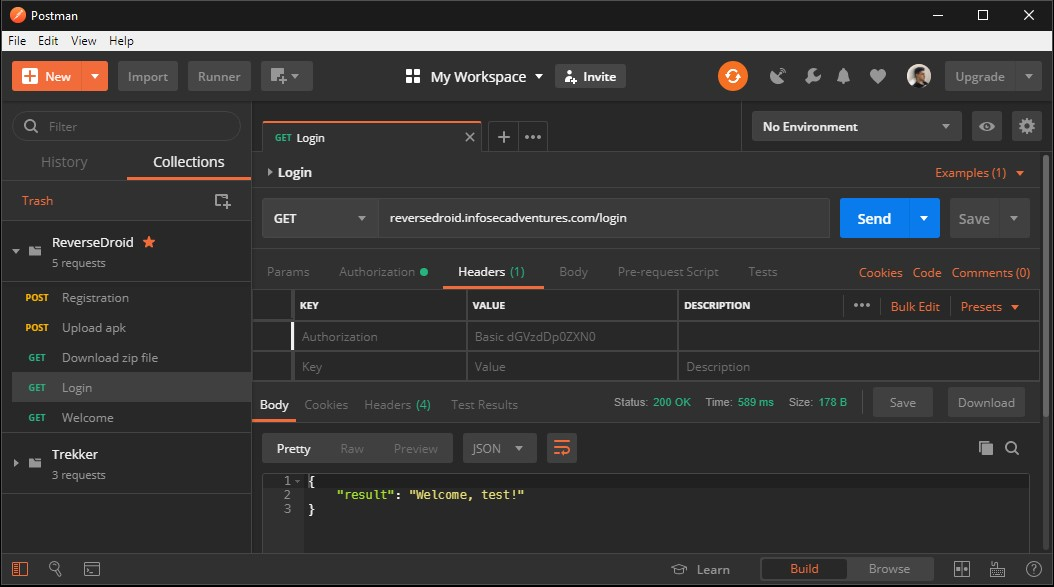
\includegraphics[width=15cm]{kepek/postman}
	\caption{Egy GET kérés és válasz a Postman alkalmazásban.}
	\label{postman}
\end{figure}

% https://www.getpostman.com/products


\chapter{Platformok}\label{platformok}

\section{A szerver kiválasztása és felépítése}

Olyan szerverre volt szükségem, ami nem túl költséges, de mégis megfelelően testreszabható és gyors tárhelyet biztosít.
A választásom a Digitial Ocean felhő szolgáltatására esett. Az oldal felületén lehetőségünk van több, úgynevezett \emph{droplet}-et létrehozni, amik nem mások mint virtuális szerverek. 
Megadhatjuk milyen disztribúciót szeretnénk telepíteni, jelen esetben én az Ubuntu Linux 18.10-es verzióját telepítettem.

\begin{figure}[!h]
	\centering
	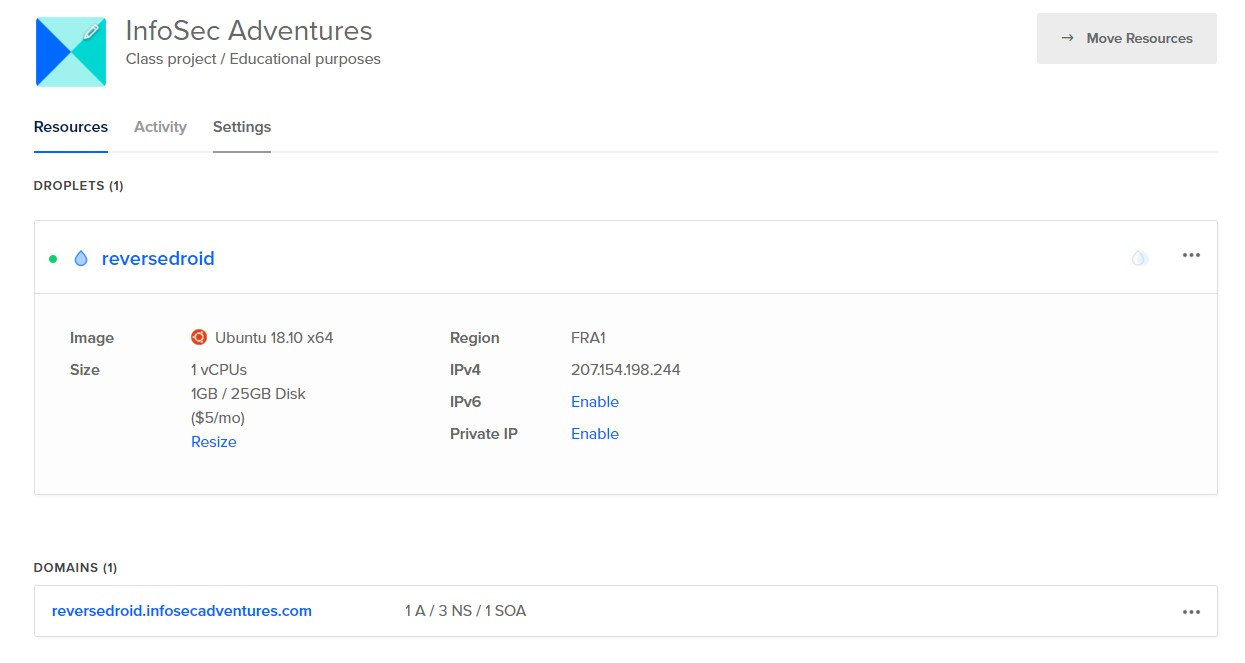
\includegraphics[width=15cm]{kepek/digitalocean}
	\caption{Droplet a Digital Ocean admin felületén.}
	\label{digitalocean}
\end{figure}

A projecthez készítettem egy subdomain-t és telepítés után a droplet IP címét hozzárendeltem ehhez a subdomain-hez.
Ezzel biztosítottam, hogy domain név alapján is elérhető legyen a szerver. Ez a \ref{namecheap} képen jól látható.

\begin{figure}[!h]
	\centering
	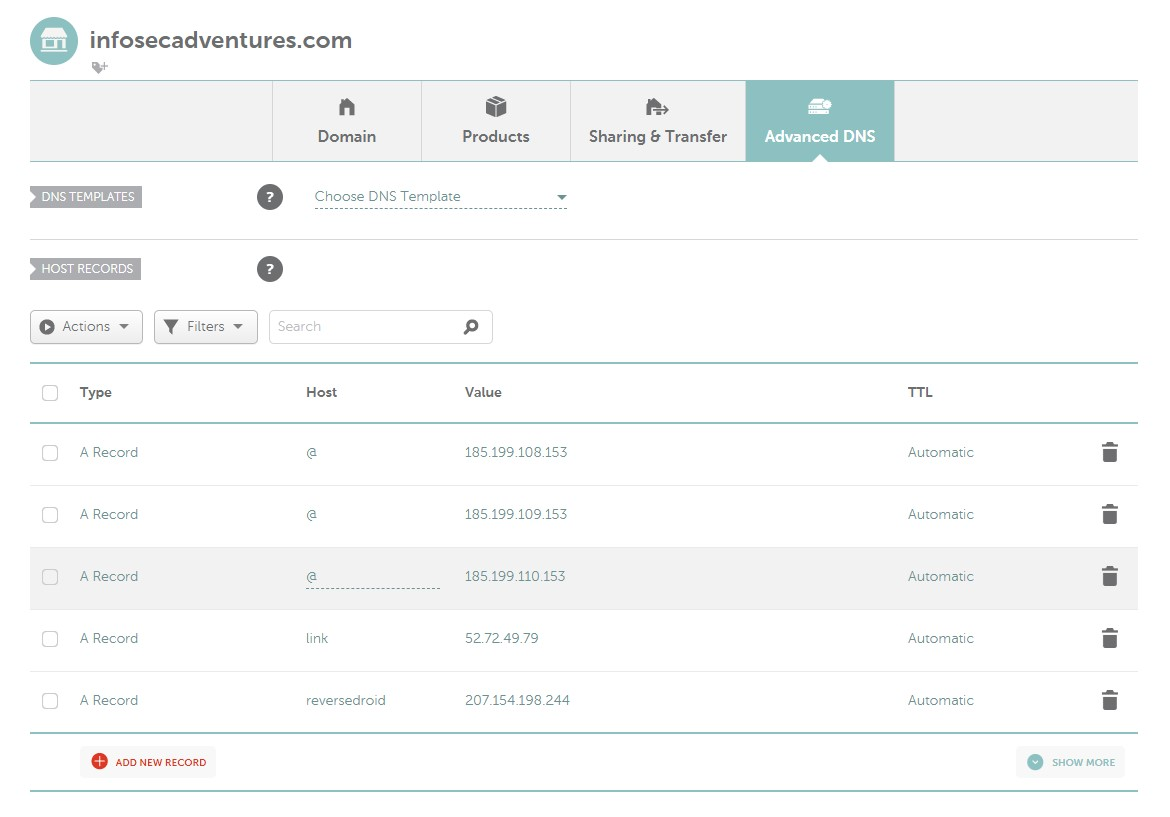
\includegraphics[width=15cm]{kepek/namecheap}
	\caption{DNS rekordok a domain beállításaiban.}
	\label{namecheap}
\end{figure}

A kész projectben nem ezt a folyamatot választottam, hanem a Digital Ocean által nyújtott ,,one-click apps'' menüben egyszerűen kiválasztottam a Docker alkalmazást és az elkészült képfájlt ezen futattam. 
Így automatizálva a szerver telepítésének folyamatát és megspórolva magának a Docker-nek a telepítését és konfigurálását.
Erről még a Szerveren használt technológiák fejezet \nameref{docker} alfejezetében bővebben írok.

\section{Mobil platform választása}

A mobilos operációs rendszerek közül az Androidot választottam. Már korábban sikerült megismerkednem az Android nyújtotta lehetőségekkel és előnyökkel.
A többi mobilos operációs rendszerrel ellentétben az Android nyílt forráskódú és a piac több mint felét uralja.
Ez annak is köszönhető, hogy 2005-ben a Google felvásárolta az Android projectet és azóta ők tartják karban.
A fejlesztő környezete elérhető mind a három fő operációs rendszerre (Linux, macOS, Windows).
Számomra ezek voltak a legnyomósabb érvek a rendszer kiválasztásában.

\chapter{Felhasznált technológiák}\label{technologiak}

\section{Verzió kezelés}

Verzió kezelésre a Git-et használtam, ami széleskörben elterjedt a fejlesztők között.
A Git egy ingyenes és nyílt-forrsákódú elosztott verzió kezelő rendszer. Úgy készült, hogy gyorsan és hatákonyan tudjon kezelni kis és nagy projekteket is egyaránt.
Már a project kezdetekor készítettem egy privát Github repository-t, hogy nyomon tudjam követni a változtatásaimat és esetleges hiba esetén visszaállítani egy korábbi verzióra.
A Github nem összetévesztendő a Git-el, mert a Git a forráskód változtatásainak kezelésére szolgál lokálisan, a Github pedig egy tárhelyet nyúlt a repository-k tárolására.
A projekt fejlesztése alatt több gépről dolgoztam és Github a segítségével biztosítani tudtam, hogy mindenhol elérjen a változtatásaimat.
Lényegében egy központi szerverként szolgált számomra.

% https://hu.wikipedia.org/wiki/Git

\section{Folyamatos integrálás}

A folyamatos integrálás egy extrém programozási gyakorlat.
A folyamatos integrálás arról szól, hogy ha egy feladat elkészült akkor azt egyből beintegráljuk a rendszerbe.
A beintegrálás után természetesen minden egység tesztnek sikeresen le kell futnia.
Több nagy cég is a \emph{CircleCi}-t használja a folyamatos integráláshoz.
Ilyen például a \emph{Facebook}, \emph{Spotify}, \emph{Kickstarter} és a \emph{GoPro}.


A CircleCi integrálható a Github-al, így kényelmesen lehet csatolni a projekt repository-ját.
A \ref{circleci} képen látható, hogy minden egyes változtatáskor lefutnak a tesztek.
Ezek a tesztek minden alkalommal egy tiszta konténerben vagy virtuális gépen futnak.
Az eredményről minden egyes alkalommal értesítést kapunk, így egyből tudhatjuk azt is, ha egy build nem futott le sikeresen.

% https://circleci.com/product/

\begin{figure}[!h]
	\centering
	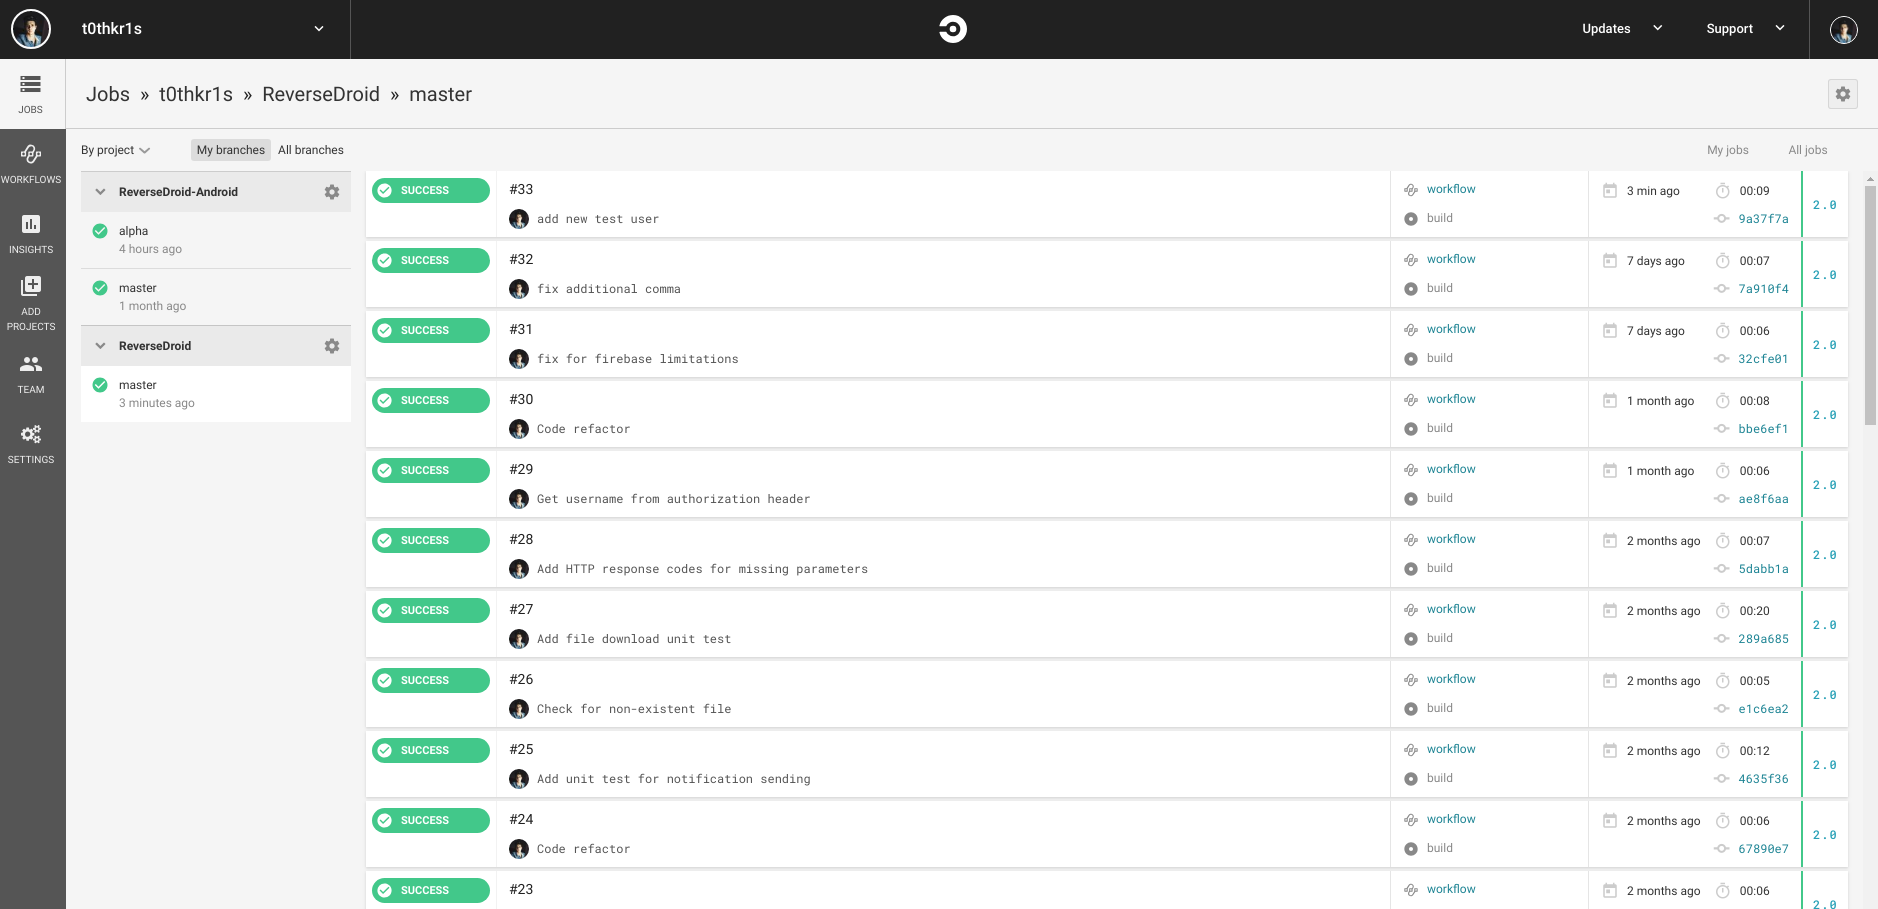
\includegraphics[width=15cm]{kepek/circle_ci}
	\caption{Sikeres project buildek a CircleCi felületén.}
	\label{circleci}
\end{figure}

\newpage

\section{Szerveren használt technológiák}

\subsection*{Flask}

A szervert a Flask webes mikro keretrendszer felhasználásával készítettem el.
A \emph{LinkedIn} és \emph{Pinteres} is említésre méltó alkalmazások, amik felhasználták ezt a keretrendszert.

\subsection*{SQLite}

Az SQLite a legtöbbet használt adatbázis motor a világon. 
Számtalan alkalmazás használja és Android-on is ez az alapértelmezett adatbázis.
Az SQLite nyílt forráskódú, így mindenki nyugodtan használhatja.

\subsection*{Pusher Beams}

A szerverről való értesítés küldéshez a Pusher Beams SDK-ját használtam.
A Beams SDK lehetővé teszi, hogy egyszerűen küldjünk push értesítést ,,érdeklődési'' körök alapján és platformtól függetlenül.
Ingyenesen és korlátlanul küldhetjük ezeket az értesítéseket.
A szerver és kliens is oldal implementációja is nagyon egyszerű és jól dokumentált, de ha mégis problémánk támadna a support is  végtelenül segítőkész.

% forrás https://docs.pusher.com/beams/reference/server-sdk-python

\subsection*{Docker}\label{docker}

A szerverhez készítettem egy Dockerfile-t és csatoltam a project Github-os repository-ját.
Ezzel elérve, hogy minden egyes változatásnál a Docker Hub újra buildelje a képfájlt.
A folyamat nagyon hasonlít a folyamatos integrálásra.

\begin{figure}[!h]
	\centering
	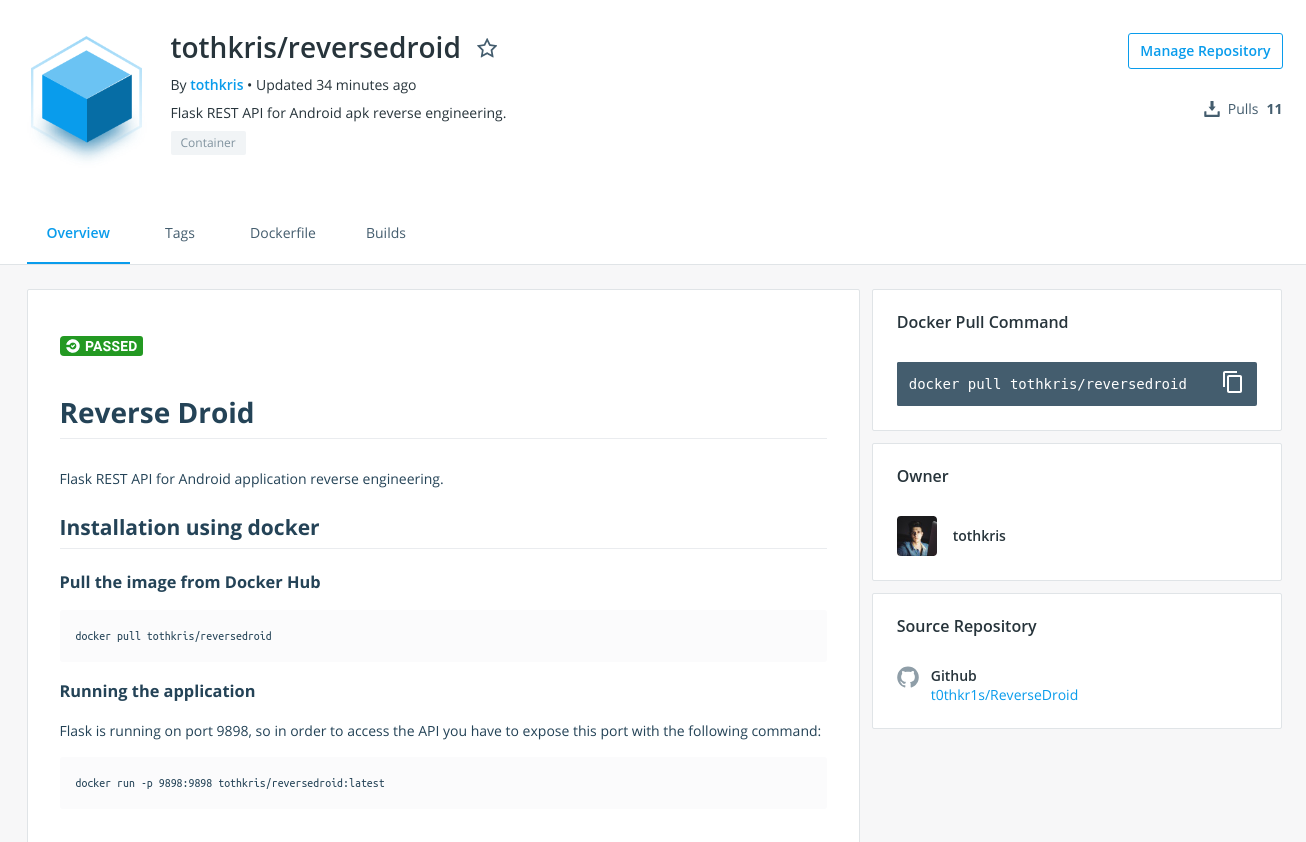
\includegraphics[width=15cm]{kepek/docker_hub}
	\caption{A szerver Docker Hub-on is elérhető.}
	\label{dockerhub}
\end{figure}

\subsection*{Tmux}

A Tmux vagy másnéven terminál multiplexer használatával több shell-t lehet futtatni.
Ez még nem is lenne túl nagy segítség, viszont ezt a folyamatot le lehet csatolni majd vissza anélkül, hogy elveszne a tartalom.
Ezen felül biztosítja, hogy a parancsok és azok kimenete kereshetők legyenek.
Az alkalmazás alapvetően a parancssorba írja a bejövő kéréseket és ez egy idő után nehezen követhető.
A Tmux nagy segítségemre volt, mivel lehetőséget adott hogy keressek a kérések között.

\subsection{jd-cmd}

Szükségem volt egy parancssorból használható Java Decompiler-re is. 

\url{https://github.com/kwart/jd-cmd}

\subsection{Apktool}

\url{https://github.com/iBotPeaches/Apktool}

\subsection{dex2jar}

Android .dex és .class fájlokkal való dolgozáskor kulcs szerepet játszott a \emph{dex2jar}. Jelen esetben nem csak egy programról beszélünk, mert valójában több eszközt foglal magába.
Az Android telepítő fájl kitömörítése után, az alkalmazás forráskódja egy \emph{classses.dex} fájlban található meg.
Ez a fájl byte kódot tartalmaz az ART számára és ezt kellett átalakítani .jar formátumba, amivel már a decompiler dolgozni tud.

\url{https://bitbucket.org/pxb1988/dex2jar}

\subsection{JSON}


\section{Androidon használt technológiák}

\subsection{AndroidX}

Az AndroidX egy nyílt forrsákódú projekt, amit az Android fejlesztői csapata használ library-k fejlesztéshez, teszteléséhez és kiadásához a Jetpack-en belül.
Az eredeti support library-hez képest az AndroidX egy jelentős fejlődés. Ahogy a support library-t is, az AndroidX-et is az Android operációs rendszertől függetlenül tudjuk használni és biztosítja a visszafelé kompatibilitást.
Az AndroidX teljesen felváltja a support library-t azáltal, hogy azonos funkciókat biztosít és új könytárakat.
Ezen felül az AndroidX a következő funkciókat tartalmazza:

\begin{enumerate}
	\item Minden csomag egy konzisztens névtérben van, ami ,,androidx''-el kezdődik.
	\item A support library-vel ellentétben az AndroidX csomagok külön vannak karbantartva és frissítve.
	\item Az összes új support library fejlesztés az AndroidX könyvtárban fog történni. Ez magába foglalja az eredeti support library fenntartását és az új Jetpack komponensek bevezetését.
\end{enumerate}


% forrás https://developer.android.com/jetpack/androidx

\subsection{OkHttp3}

\subsection{Okio}

\subsection{Pusher Beams}

% forrás https://docs.pusher.com/beams/reference/android


\subsection{Firebase Messaging}

\subsection{Room}

A Room egy absztrakciós réteget nyújt az SQLite adatbázishoz, ezzel lehetővé téve az egyszerűbb és hatékonyabb adatbázis elérést.
A Room segítségével sokkal egyszerbben tudtam kezelni az SQLite adatbázist, mert nem kellett adatbázist leíró osztályt és hosszú lekérdezéseket írnom.
Ami külön tetszett benne, hogy az SQL utasításokat fordítási időben ellenőrzi.
Annotációk segítségével tudjuk összekötni a Java POJO osztályokat az SQLite adatbázissal.

\subsection{CodeView}

A forrás kód megjelenítését nem lett volna célszerű nulláról felépíteni, ezért inkább kész megoldások után néztem.
Több megfelelő forrás kód megjelenítő könyvtárat találtam, így funkciók alapján kellett döntenem, hogy melyiket válasszam.

\begin{figure}[!h]
	\centering
	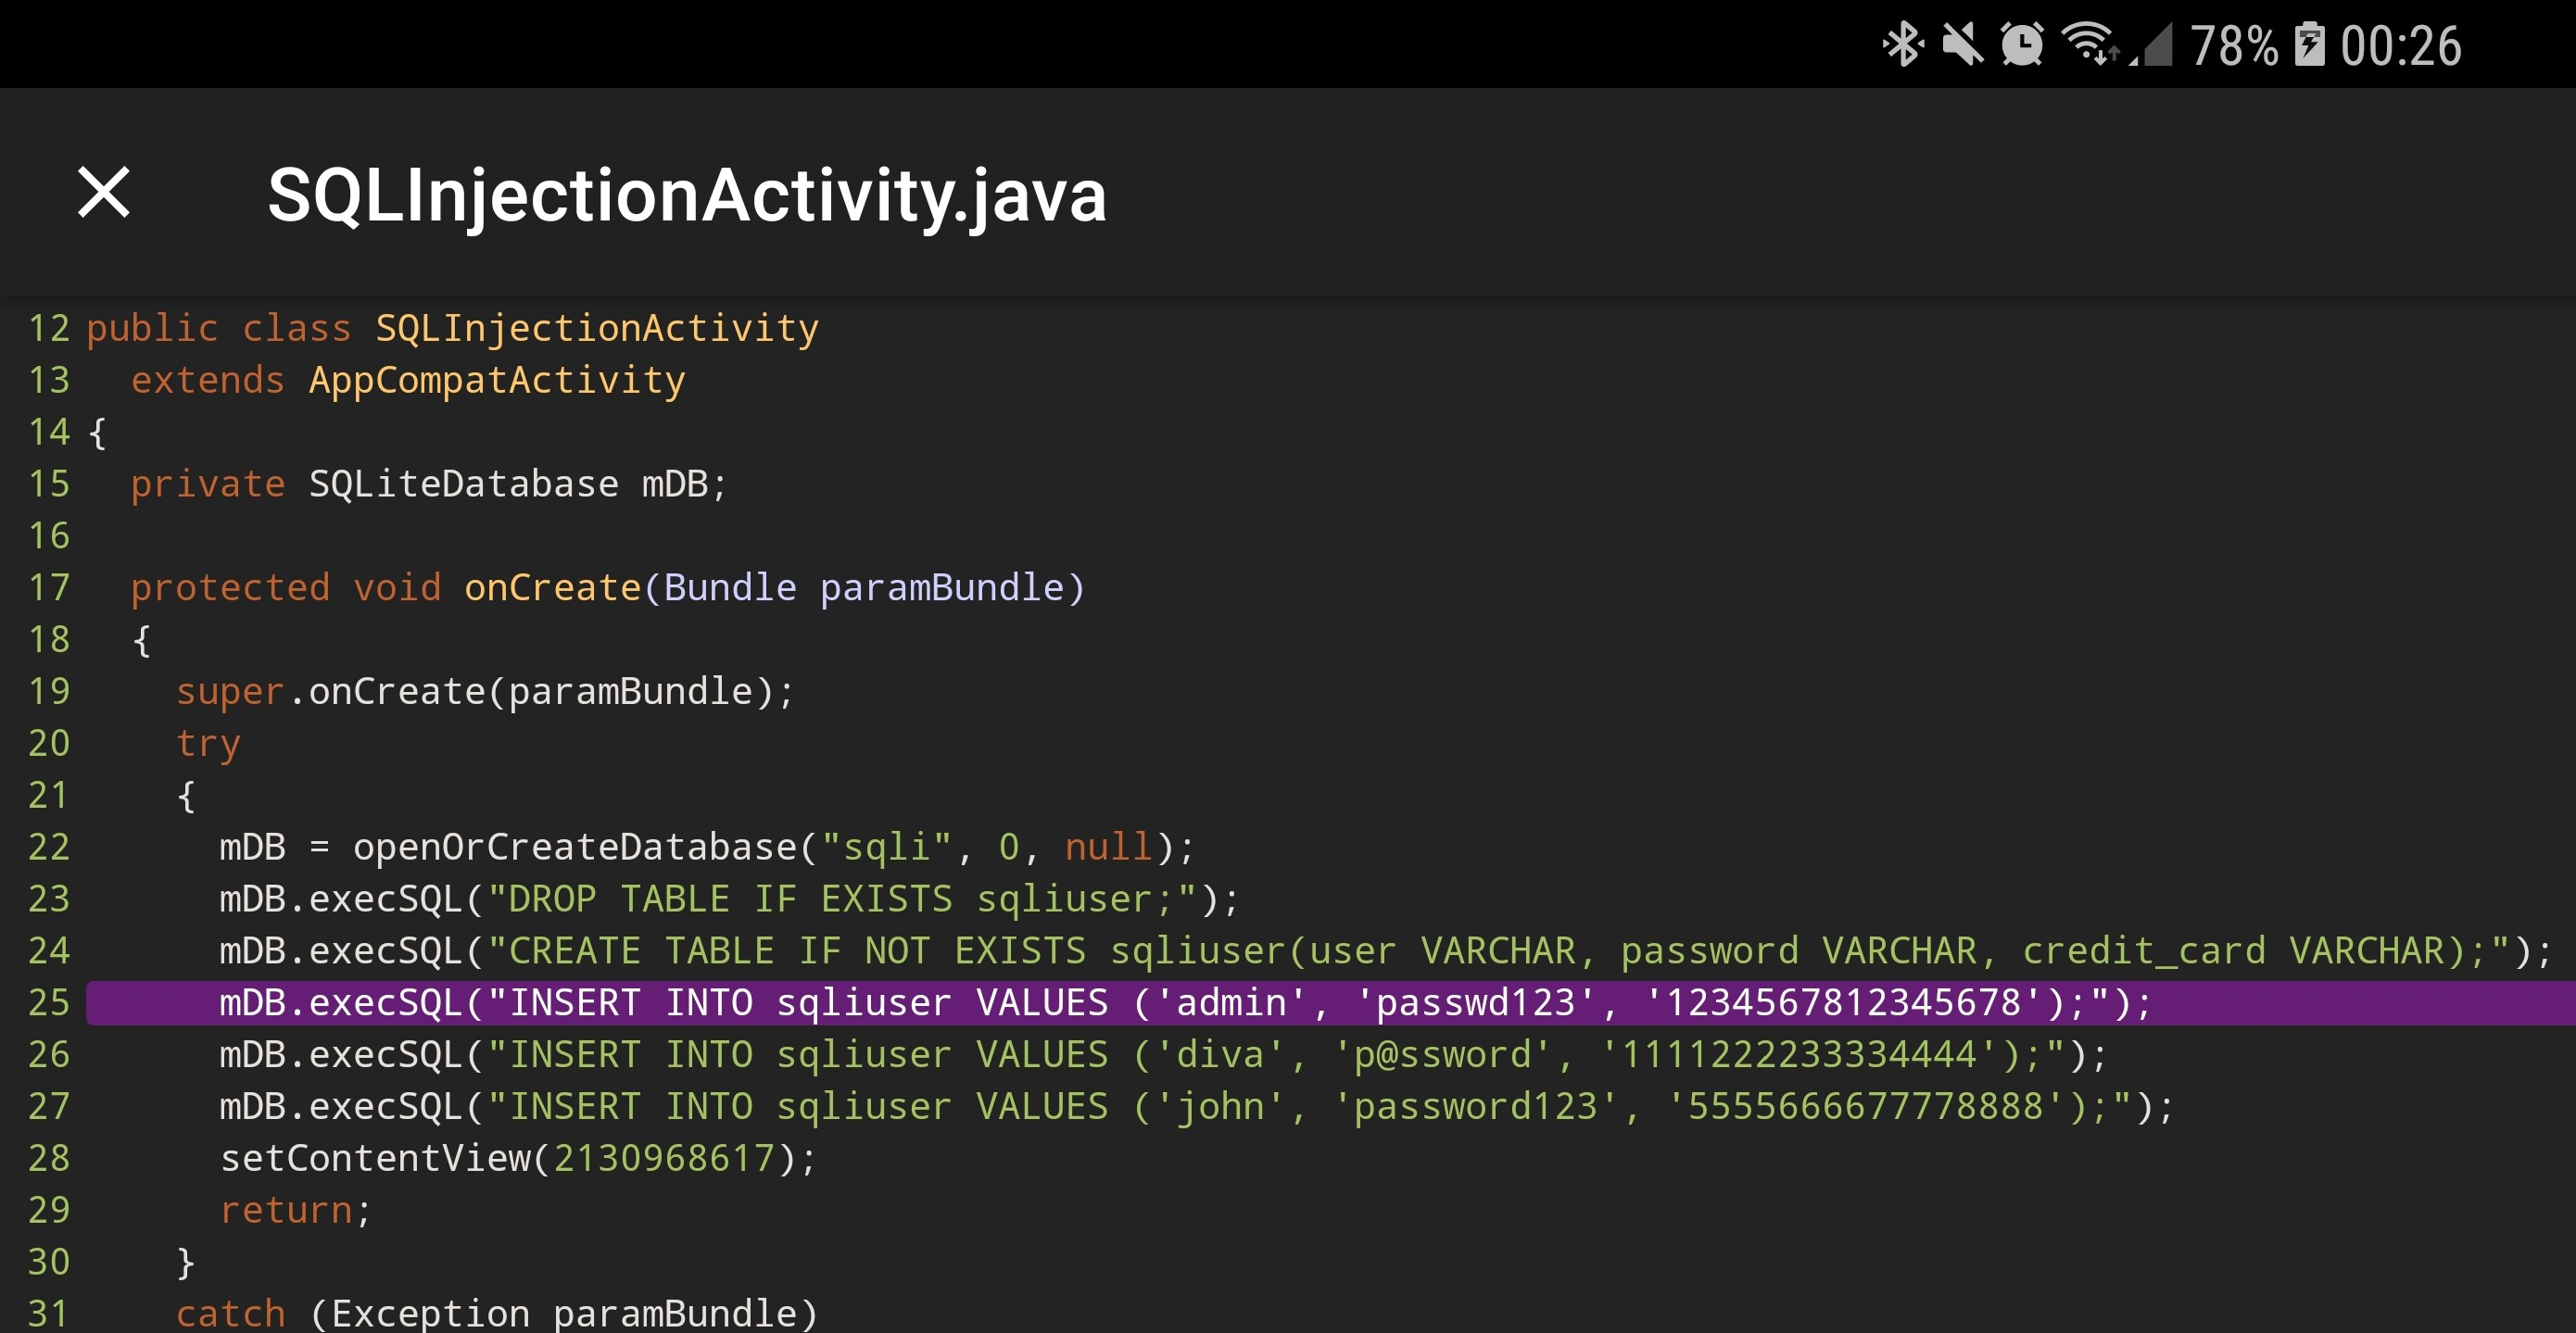
\includegraphics[width=15cm]{kepek/code_view}
	\caption{A vissza fejtett forrás kód megjelenítése.}
	\label{dockerhub}
\end{figure}

\subsection{Espresso}

\subsection{Material Design 2.0}

\chapter{Teszteléshez felhasznált eszközök és források}\label{teszteles}

\section{Sérülékeny Android alkalmazások}

A teszteléshez keresnem kellett olyan sérülékeny alkalmazásokat, amelyeken jól lehet demonstrálni a visszafejtést.
Minden alkalmazás, amit itt megemlítek nyílt forrás kódú és kimondottan erre a céltra készítették őket.
Ez azért is jó, mert a visszafejtett kódot össze lehet hasonlítani az eredetivel és megnézni mennyire volt hatékony a visszafejtési folyamat.
A következő lista tartalmazza a teszteléshez felhasznált szándékosan sérülékeny alkalmazásokat.

\begin{itemize}
	\item \href{https://github.com/payatu/diva-android}{Diva}
	\item \href{https://github.com/as0ler/Android-Examples}{Sieve}
	\item \href{https://github.com/htbridge/pivaa}{Pivaa}
	\item \href{https://github.com/t0thkr1s/frida-demo}{Frida}
\end{itemize}

\chapter{Megvalósított funkciók}\label{funkciok}

\section{Bejelentezés}

\section{Regisztráció}

\section{Kijelentkezés}

\section{Adatok törlése}

\section{Fájl feltöltés}

\section{Fájl letöltés}

\section{Navigáció a fájlrendszerben}

A letöltött és kitömörített projektek az alkalmazás mappájában kerülnek.
Ezzel alapvetően nincs is semmi probléma, csak ha megszeretnénk nézni a fájlokat, akkor elkellene hagynunk az alkalmazást.
Ez pedig rossz felhasználói élményhez vezetett volna.
Ennek megoldására megvalósítottam egy nagyon egyszerű fájl rendszer navigációt, de ezt csak az alkalmazás mappájában tettem lehetővé.
Így kitömörítés után egyszerűen és gyorsan elérhetővé válik a project a felhasználó számára.
Részleteit tekintve csak a fájl nevét, módosítás dátumát és a fájl méretét jelenítettem meg.

\section{Értesítések}

Az értesítések küldése és fogadása szintén egy kulcs fontosságú része az alkalmazásnak.
A fájlok letöltése és kitömörítése mérettől, valamint hálózati kapcsolattól függően időt vesz igénybe.

A szerveren történő visszafejtés az a folyamat, ami jelentős időtartamot igényel.

\chapter{Továbbfejlesztési lehetőségek}\label{lehetosegek}

Úgy gondolom, hogy sokkal nagyobb piaci érték rejlik ebben az alkalmazásban.
A jövőben is szeretném folytatni a fejlesztést.
Szeretnék több figyelmet fordítani a biztonságra és hatékonyságra.
Gondolok itt a biztonságos kommunikációra TLS-es keresztül és a harmadik féltől származó könyvtárak csökkentésére.
A kód visszafejtése végén egy összegző report is hasznos lehet a felhasználó számára, ami tartalmazhatja a feldolgozott fájlok számát.
Egy esetleges forrás kód elemző 

\chapter{Tapasztalatok}\label{tapasztalatok}

Úgy érzem elértem a célom ezzel a projecttel és sokat sikerült tanulnom a folyamatban.
Új technológiákat ismertem meg és használtam.
Természetesen nem volt minden magától értetődő és jó pár nehézséggel is találkoztam.


\begin{thebibliography}{1}
\bibitem{statista} \textsc{ONLINE}: Number of mobile phone users worldwide from 2015 to 2020, \url{https://www.statista.com/statistics/274774/forecast-of-mobile-phone-users-worldwide}
\bibitem{androidstudio} \textsc{ONLINE}: Everything you need to build on Android \url{https://developer.android.com/studio/features.html}
\bibitem{pycharm} \textsc{ONLINE}: PyCharm Features \url{https://www.jetbrains.com/pycharm/features/}
\end{thebibliography}
\end{document}
